\documentclass{article}
\usepackage[utf8]{inputenc}
\usepackage{amsmath,amsthm,amssymb}

\title{Solution Mannual for Supplyment Psets of MIT OCW 18.02SC Fall 2010}
\author{Lu YuXun}
\date{February 2017}

\usepackage{natbib}
\usepackage{graphicx}

\begin{document}

\maketitle

\section{Psets 1}
\subsection{1. Vectors and Matrices}
\textbf{1A-12*} Label the four vertices of a parallelogram in counterclockwise order as OPQR. Prove that the line segment from O to the midpoint of PQ intersects the diagonal PR in a point X that is 1/3 of the way from P to R.
\begin{figure}[htp!]
    \centering
    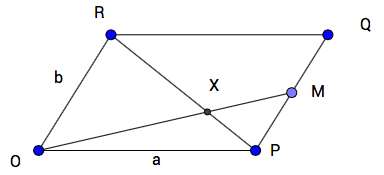
\includegraphics[width=50mm,scale=0.5]{Figure/1A-12.png}
    \caption{1A-12 Figure}
    \label{1A-12 Figure}
\end{figure}
\begin{proof}
Suppose $\vec{OP} = \mathbf{a}$ and $\vec{OR} = \mathbf{b}$.
\end{proof}

\end{document}
